\section{Udvælgelse af skalaer}
\label{ParametreDatabehandlingSkalaer}
%
OBS:NOGET OM HVORDAN PARAMETRENE ER "FUNDET" \\
Ud fra de opstillede parametre, opstilles der skalaer, ved at gennemgå alle sætningerne markeret med S (for Scale). Kravet for opstilling af en skala er, at det er muligt at ændre på den specifikke parametre skalaen beskriver. Formålet er at opstille den optimale skala for hvert enkelt parameter, der er derfor ikke fastsat én specifik skala type på forhånd. 

Det vurderes at en bipolær skala er mest beskrivende da den har den største spænd og denne vil derfor fortrækkes, i tilfælde hvor der findes både en bipolær og unipolær. \blankline
%
OBS: Nogen af de orange sticky notes fra det foregående afsnit bliver slået sammen, fordi de egentlig siger det samme og hører under det samme emne. \blankline
%
OBS: ANTALLET AF SKALAER ER REDUCERET FRA 30 TIL 24
%
OBS: Hvis potentielle skala spørgsmål fra det forrige afsnit er sat sammen til en "endelig" skala er det gjort på baggrund af egne vurderinger og der er derfor ikke opsat nogle kriterier for sammensætningen, udover at det skal dække over det samme.\blankline
%
\textbf{INTERAGERER IKKE MED R}\\
Det ene potentielle skala spørgsmål \textit{Er det let at undgå R}, der var til \textit{Interagerer ikke med R}, er hører nu under \textit{Jeg synes at robotten er anmassende}.\blankline
%
\textbf{SKÆRMEN VIRKER IKKE}\\
Dette vil ikke være en skala, der "behandles" på samme måde som de andre, men en skala, der kan være med til at undersøge hvorvidt det har en indflydelse. Skalaen vil derfor ikke indgå blandt de andre skalaer, men være en af de sidste spørgsmål testpersonerne i den næste test får. 
%
\begin{figure}[H]
\centering
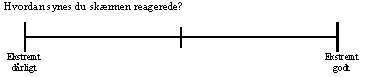
\includegraphics[width =\textwidth]{Figure/UdvalgteSkalaer/SkaermensReaktion} 
\caption{NY.}
\label{fig:SkalaSkaermensReaktion}
\end{figure}
\noindent
%
\textbf{R KAN ASSISTERE MENNESKER}\\
%
\begin{figure}[H]
\centering
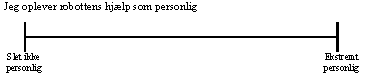
\includegraphics[width =\textwidth]{Figure/UdvalgteSkalaer/PersonligHjaelp} 
\caption{NY.}
\label{fig:SkalaPersonligHjaelp}
\end{figure}
\noindent
%
Jeg føler R kan hjælpe mig, R kan hjælpe mig så jeg ikke behøver at spørger personale slåes sammen til: Jeg føler at R kan hjælpe mig. Hvor \textit{ Jeg kan bruge R til at finde rundt i L slåes sammen til} tidligere blev slået sammen med at \textit{Jeg føler R kan hjælpe mig}.
%
\begin{figure}[H]
\centering
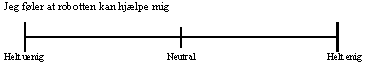
\includegraphics[width =\textwidth]{Figure/UdvalgteSkalaer/RobottenKanHjaelpe} 
\caption{NY.}
\label{fig:SkalaRKanHjaelpe}
\end{figure}
\noindent
%
\textbf{R'S VÆREMÅDE}\\
%
\begin{figure}[H]
\centering
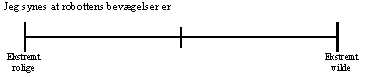
\includegraphics[width =\textwidth]{Figure/UdvalgteSkalaer/BevaegelserR} 
\caption{NY.}
\label{fig:SkalaBevaegelserR}
\end{figure}
\noindent
%
%
\begin{figure}[H]
\centering
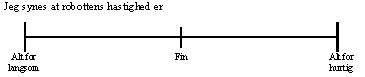
\includegraphics[width =\textwidth]{Figure/UdvalgteSkalaer/HastighedR} 
\caption{NY.}
\label{fig:SkalaHastighedR}
\end{figure}
\noindent
%
%
\begin{figure}[H]
\centering
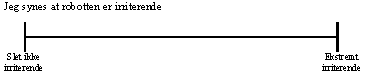
\includegraphics[width =\textwidth]{Figure/UdvalgteSkalaer/Irriterende} 
\caption{NY.}
\label{fig:SkalaIrriterende}
\end{figure}
\noindent
%
Nedenstående skala er slået sammen af: \textit{Jeg synes at R er levende} fra kategori: \textit{R's væremåde} og \textit{Jeg synes at R ser menneskelig ud} fra kategori: \textit{R's udseende}, hvor \textit{Jeg foretrækker at R ser menneskelig ud} blev slået sammen.
%
\begin{figure}[H]
\centering
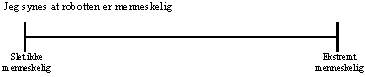
\includegraphics[width =\textwidth]{Figure/UdvalgteSkalaer/MenneskeligR} 
\caption{NY.}
\label{fig:SkalaMenneskeligR}
\end{figure}
\noindent
%
Nedenstående skala er slået sammen af: \textit{Jeg synes at R er anmassende}, \textit{Jeg synes at R er intimiderende} (fra kategori: \textit{Henvendelse}) og \textit{Er det let at undgå R} fra kategori: \textit{Interagerer ikke med R} 
%
\begin{figure}[H]
\centering
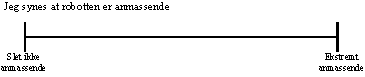
\includegraphics[width =\textwidth]{Figure/UdvalgteSkalaer/Anmassende} 
\caption{NY.}
\label{fig:SkalaAnmassende}
\end{figure}
\noindent
%
\textbf{HENVENDELSE}\\
%
\begin{figure}[H]
\centering
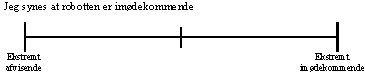
\includegraphics[width =\textwidth]{Figure/UdvalgteSkalaer/Imoedekommende} 
\caption{NY.}
\label{fig:SkalaImoedekommende}
\end{figure}
\noindent
%
%
\begin{figure}[H]
\centering
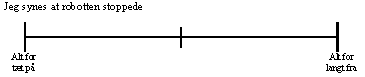
\includegraphics[width =\textwidth]{Figure/UdvalgteSkalaer/RStoppede} 
\caption{NY.}
\label{fig:SkalaRStoppede}
\end{figure}
\noindent
%
%
\begin{figure}[H]
\centering
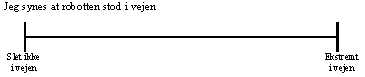
\includegraphics[width =\textwidth]{Figure/UdvalgteSkalaer/RobottenErIVejen} 
\caption{NY.}
\label{fig:SkalaRerIVejen}
\end{figure}
\noindent
%
%
\begin{figure}[H]
\centering
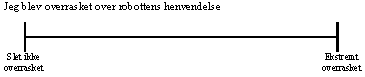
\includegraphics[width =\textwidth]{Figure/UdvalgteSkalaer/OverrasketOverR} 
\caption{NY.}
\label{fig:SkalaOverrasketOverR}
\end{figure}
\noindent
%
\textbf{R'S UDSEENDE}\\
Fjerner \textit{Jeg kan godt lide R's udseende} fordi det formentlig er en overkategori til sej, sjov, sød, elegant, så hvis de rates højt er det formentlig et udtryk for at de også godt kan lide robottens udseende, hvorhvis sej, sjov, sød mm. rates dårligt er det et udtryk for at de ikke kan lide R's udseende. Så parameteren bliver målt indirekte, ved andre parametre.
%
\begin{figure}[H]
\centering
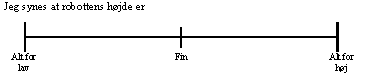
\includegraphics[width =\textwidth]{Figure/UdvalgteSkalaer/HoejdeR} 
\caption{NY.}
\label{fig:SkalaHoejdeR}
\end{figure}
\noindent
%
%
\begin{figure}[H]
\centering
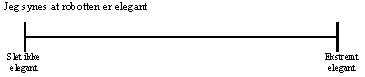
\includegraphics[width =\textwidth]{Figure/UdvalgteSkalaer/ElegantR} 
\caption{NY.}
\label{fig:SkalaElegantR}
\end{figure}
\noindent
%
\textbf{INTERESSE FOR R}\\
\textit{Jeg synes at R er spændende} og \textit{R fangede min opmærksomhed}, bliver slået sammen til nedenstående. Tidligere blev \textit{Jeg blev nysgerrige da jeg så R} slået sammen med \textit{Jeg synes at R er spændende}.
%
\begin{figure}[H]
\centering
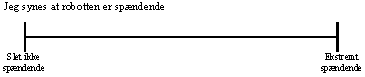
\includegraphics[width =\textwidth]{Figure/UdvalgteSkalaer/RerSpaendende} 
\caption{NY.}
\label{fig:SkalaRerSpaendende}
\end{figure}
\noindent
%
\textbf{POSITIV OVERFOR R}\\
%
\begin{figure}[H]
\centering
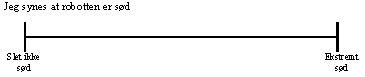
\includegraphics[width =\textwidth]{Figure/UdvalgteSkalaer/SoedR} 
\caption{NY.}
\label{fig:SkalaSoedR}
\end{figure}
\noindent
%
%
\begin{figure}[H]
\centering
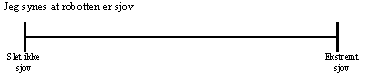
\includegraphics[width =\textwidth]{Figure/UdvalgteSkalaer/SjovR} 
\caption{NY.}
\label{fig:SkalaSjovR}
\end{figure}
\noindent
%
%
\begin{figure}[H]
\centering
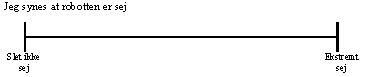
\includegraphics[width =\textwidth]{Figure/UdvalgteSkalaer/SejR} 
\caption{NY.}
\label{fig:SkalaSejR}
\end{figure}
\noindent
%
%
\begin{figure}[H]
\centering
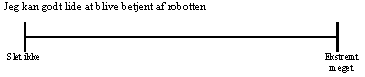
\includegraphics[width =\textwidth]{Figure/UdvalgteSkalaer/BetjeningAfR} 
\caption{NY.}
\label{fig:SkalaBetjeningAfR}
\end{figure}
\noindent
%
\textbf{KENDSKAB TIL TEKNOLOGI}\\
%
\begin{figure}[H]
\centering
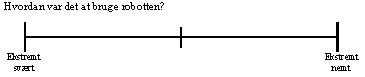
\includegraphics[width =\textwidth]{Figure/UdvalgteSkalaer/HvordanVarDetAtBrugeR} 
\caption{NY.}
\label{fig:SkalaHvordanVarDetAtBrugeR}
\end{figure}
\noindent
%
%
\begin{figure}[H]
\centering
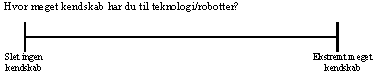
\includegraphics[width =\textwidth]{Figure/UdvalgteSkalaer/KendskabTilTeknologi} 
\caption{NY.}
\label{fig:SkalaKendskabTilTeknologi}
\end{figure}
\noindent
%
\textbf{TILLID TIL R}
%
\begin{figure}[H]
\centering
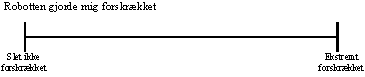
\includegraphics[width =\textwidth]{Figure/UdvalgteSkalaer/Forskraekket} 
\caption{NY.}
\label{fig:SkalaForskraekket}
\end{figure}
\noindent
%
%
\begin{figure}[H]
\centering
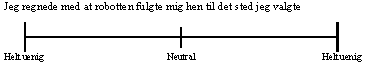
\includegraphics[width =\textwidth]{Figure/UdvalgteSkalaer/RobottenFulgteMigDetRigtigeStedHen} 
\caption{NY.}
\label{fig:SkalaRFulgteMigDetRigtigeStedHen}
\end{figure}
\noindent
%
%
\begin{figure}[H]
\centering
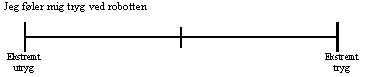
\includegraphics[width =\textwidth]{Figure/UdvalgteSkalaer/TrygVedR} 
\caption{NY.}
\label{fig:SkalaTrygVedR}
\end{figure}
\noindent
%
